\chapter{Giới thiệu đề tài}
\section{Đặt vấn đề}
Trong y khoa, trực quan hoá dữ liệu là một nhu cầu thiết thực để tăng độ chính xác trong chuẩn đoán và điều trị nhiều loại tổn thương khác nhau của bệnh nhân. Đặc biệt đối với những loại chấn thương và bệnh lý ở các cơ quan nội tạng nằm bên trong cơ thể khi mà những bộ phận này không thể được quan sát trực tiếp bằng mắt thường, việc mô phỏng lại cơ quan đó thông qua các thiết bị kỹ thuật càng trở nên thiết yếu hơn. \\
Trước đây, phương pháp chụp X-quang cho phép hiển thị được hình chiếu của các bộ phận bên trong cơ thể nhờ vào mức độ hấp thụ khác nhau của các loại mô đối với tia X. Về sau, nhờ ứng dụng nhiều công nghệ kỹ thuật tiên tiến, người ta đã có thể chụp được nhiều ảnh X-quang từ nhiều hướng khác nhau rồi từ đó sử dụng các thiết bị vi tính để tính toán ra các ảnh cắt lớp của một vùng bất kỳ trên cơ thể bệnh nhân, kỹ thuật chụp ảnh này chính là Computed Tomography (CT).\\
Mặc dù đã đạt được một bước tiến đáng kể để có thể tái tạo được những hình ảnh các cơ quan nội tạng của bệnh nhân mà không cần mổ, song muốn có được một cái nhìn tổng thể ba chiều của một cơ quan bất kỳ vẫn cần sự can thiệp lớn của các bác sĩ. Hình khối ba chiều của một cơ quan nội tạng được xây dựng từ các ảnh cắt lớp của riêng bộ phận đó. Để có được ảnh cắt lớp riêng của một bộ phận từ ảnh CT cần các bác sĩ thực hiện nhận diện và phân đoạn chính xác bộ phận đó trên từng lát cắt của ảnh. Thông thường một ảnh CT ba chiều sẽ có số lát cắt từ một trăm đến bai trăm, mộ số ảnh chi tiết hơn có thể lên tới chín trăm lát cắt. Phải tiến hành phân đoạn trên một ảnh có nhiều lát cắt là thách thức lớn nhất của các bác sĩ khi muốn trực quan hoá một cơ quan nằm bên trong cơ thể lên không gian ba chiều.\\
Để giải quyết vấn đề về phân đoạn số lát cắt ba chiều lớn, nhiều giải pháp phân đoạn tự động đã được nghiên cứu và sử dụng. Tuy nhiên độ chính xác của các phương pháp này không cao do độ tương phản của các cơ quan rất giống nhau, đặc biệt là ở lồng ngực. Các phương pháp đạt hiệu quả cao hiện tại thường là các giải pháp bán tự động và cần sự can thiệp của đôị ngũ y bác sĩ.
\section{Mục tiêu đề tài}
Trong luận văn tốt nghiệp này, chúng tôi sẽ xây dựng một giải pháp phân đoạn tự động trên cơ sở của mạng học sâu để có thể trích xuất được thông tin bề mặt và trực quan hoá ba chiều cơ quan nội tạng từ ảnh CT chứa cơ quan đó. Để đánh giá giải pháp được xây dựng ở đề tài này, chúng tôi sẽ tiến hành so sánh mô hình của chúng tôi với các mô hình khác đã được các Luận văn tốt nghiệp trước trình bày. Bên cạnh đó chúng tôi cũng sẽ sử dụng các công cụ và tập dữ liệu đã được công khai có tính khách quan cao để đánh giá kết quả của mô hình được phát triển trong đề tài này. Và cuối cùng, chúng tôi sẽ xây dựng một ứng dụng cho phép phân đoạn tự động lá gan từ ảnh CT được người dùng đưa vào và hiển thị mô hình ba chiều cùng với ước lượng thể tích của lá gan đó.

\begin{figure*}
  \centering
  \subfigure[Ảnh CT lồng ngực]{%
    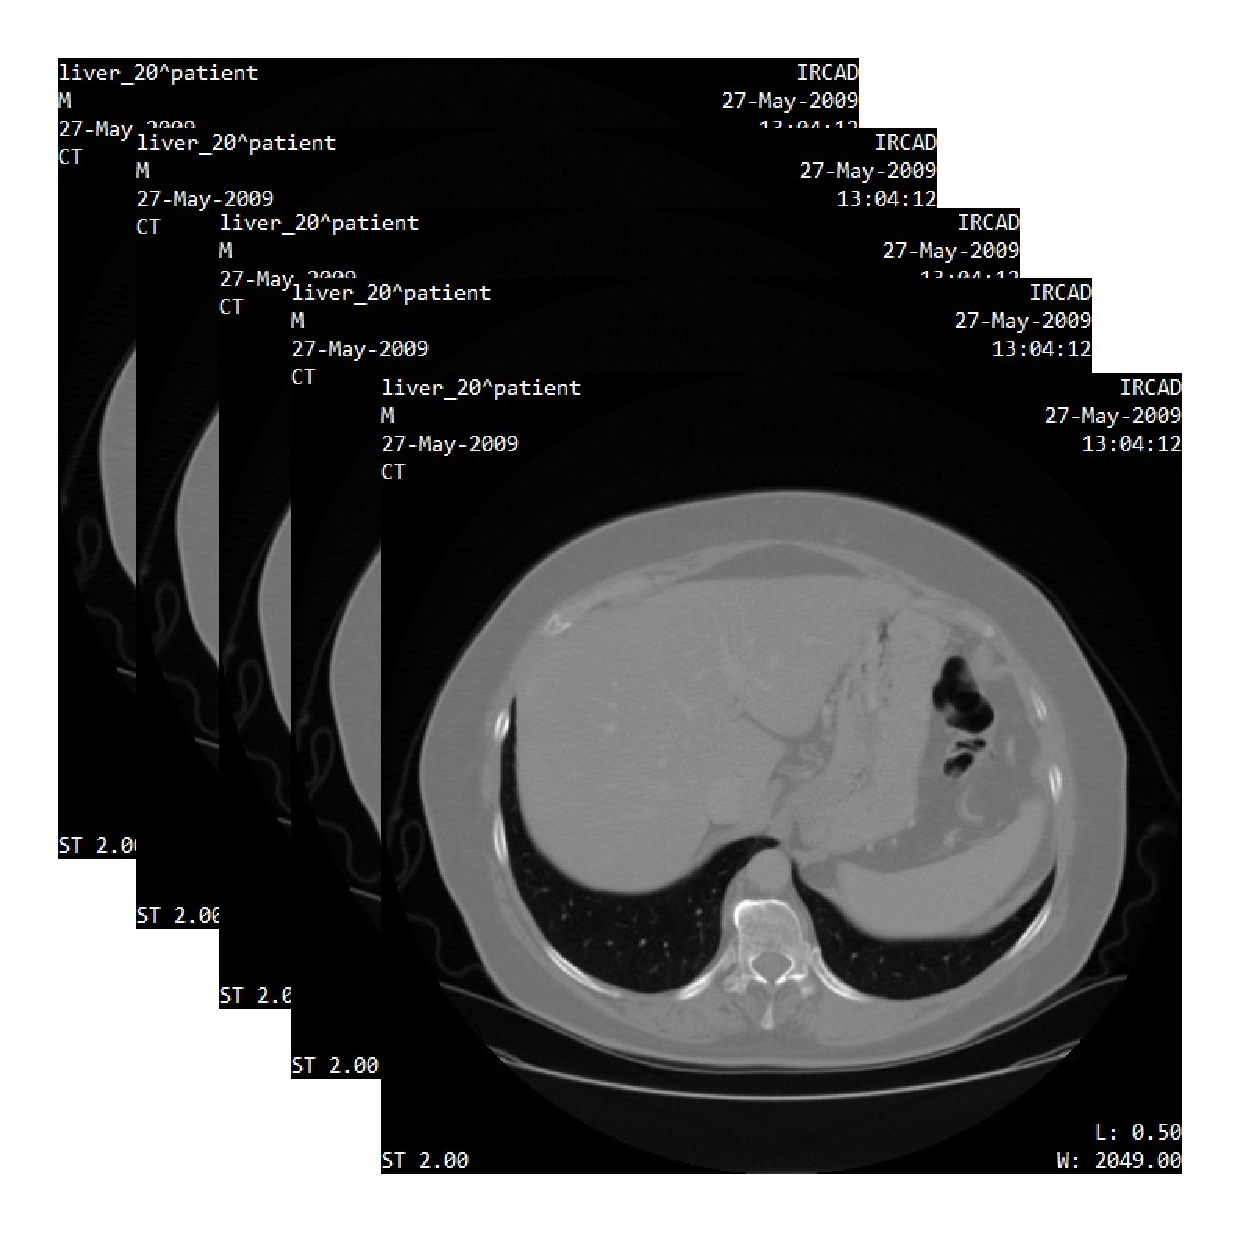
\includegraphics[width=0.3\textwidth]{Images/image5.pdf}%
    \label{fig:image5}%
    }
    \subfigure[Ảnh phân đoạn lá gan]{%
    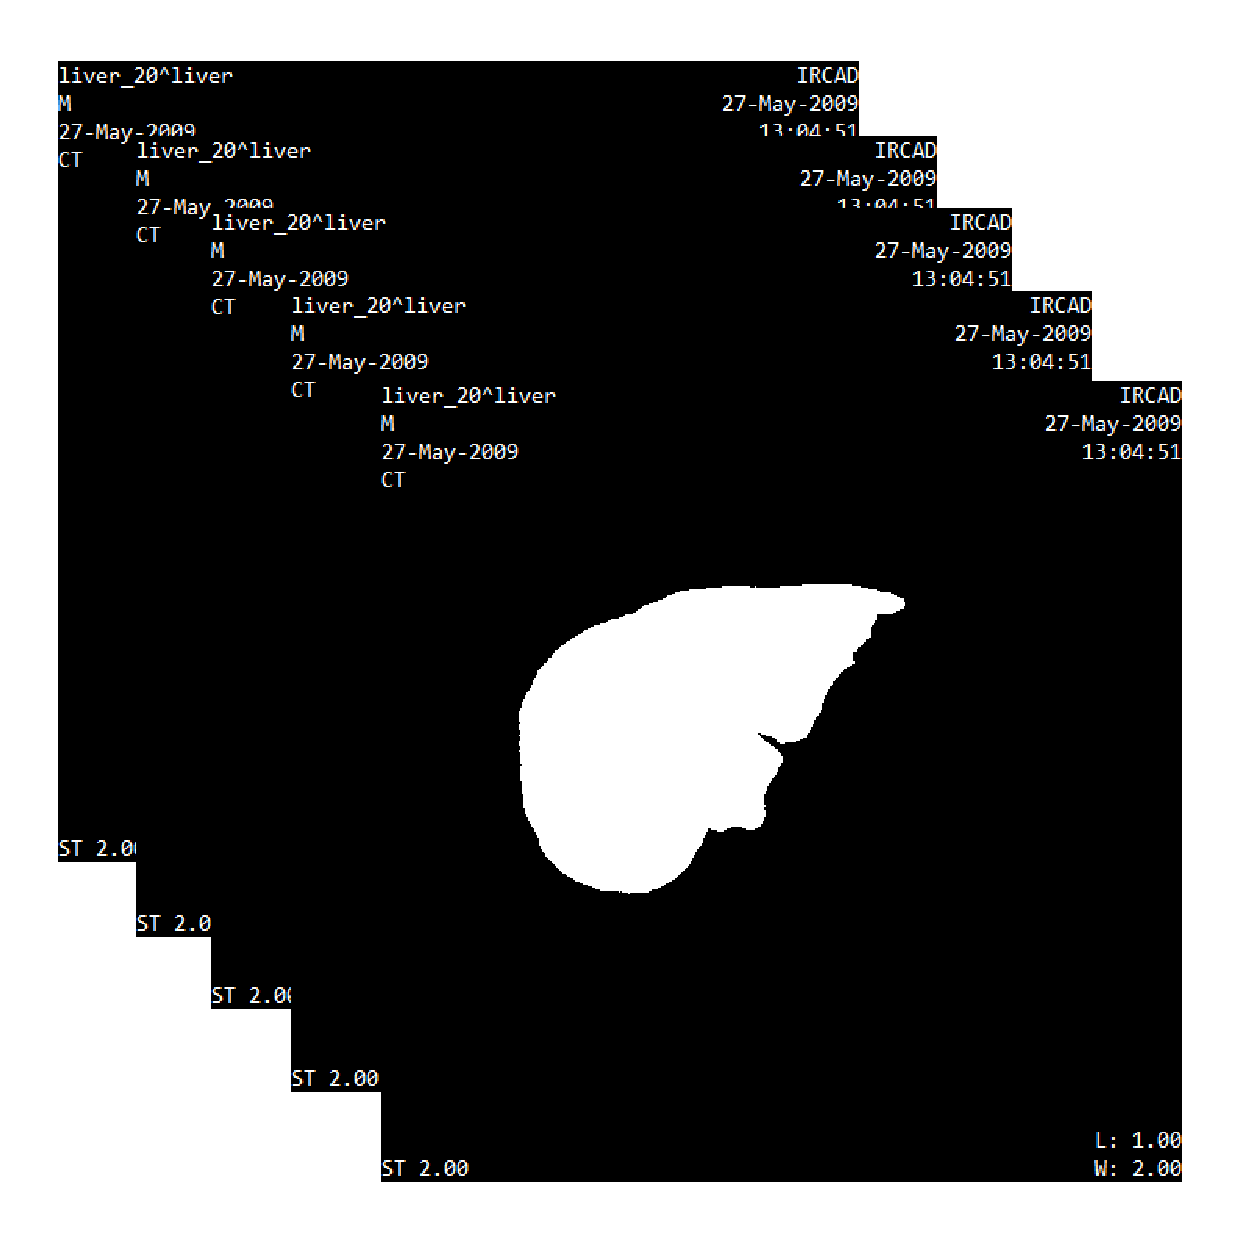
\includegraphics[width=0.3\textwidth]{Images/label5.pdf}%
    \label{fig:b}%
    }
    \subfigure[Ảnh lá gan 3 chiều]{%
    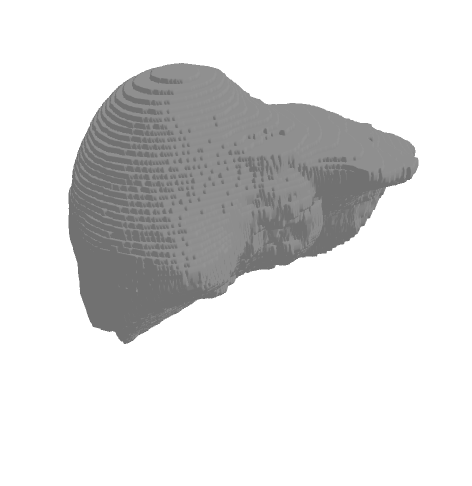
\includegraphics[width=0.3\textwidth]{Images/liver3d.png}%
    \label{fig:c}%
    }% 
  \caption{Minh hoạ quá trình xây dựng lá gan 3 chiều từ ảnh CT lồng ngực}
  \label{fig:ab}
\end{figure*}
\section{Phạm vi thực hiện}
Trong khuôn khổ của một Luận văn tốt nghiệp, chúng tôi sẽ giới hạn lại phạm vi nghiên cứu phù hợp để có thể đảm bảo được tính ứng dụng của đề tài và tính khách quan khi đánh giá mô hình được xây dựng với các mô hình khác. Ở đề tài này, chúng tôi sẽ tập trung vào xây dựng mô hình lá gan từ ảnh CT chụp lồng ngực bằng phương pháp chính là học sâu. Mô hình của chúng tôi sẽ được đánh giá với mô hình hai mô hình của anh Đàm Vũ Duy và của nhóm hai anh Bùi Hồng Thiên Nhật - Phạm Huỳnh Sơn. Giải pháp của chúng tôi cũng sẽ được đánh giá với các tập dữ liệu đã được sử dụng tại các hội nghị về xử lý ảnh y khoa có uy tín cáo SLiver07 \cite{website:slvier07}, 3Dircadb \cite{website:data_3DIRCADb}, LiTS2017 \cite{website:LiTS}.